\chapter{Data collection and pre-processing}
\label{chap:data}

In the crypto-currency domain, real-time price data is, for most exchanges, freely available. Historical data is oftentimes limited with respect to how far back into past the data is being provided. However, continuously recording real-time data results in a complete historical data set from the time when recording was started and provides the desired data set for this research.

A historical limit order book consisting of states which stores all the bids and asks posted from traders in the past is commonly referred to as a \textit{complete order book}.
The process to accumulate the data and build the order book is illustrated in a high level pipeline in Figure \ref{fig:data-pipeline} below.
\begin{figure}[H]
    \centering
    \makebox[\linewidth]{
        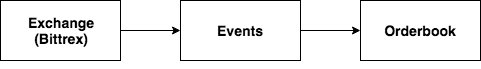
\includegraphics[width=8cm]{data-pipeline.png}
    }
    \caption{Data collection pipeline}
    \label{fig:data-pipeline}
\end{figure}
\hfill
In this chapter we explain the details of the collection process process and subsequently how a historical order book was formed thereof.
We further analyze a collected data set and visualize its key elements.

\section{Collection}

There are various ways in order to build a copy of a historical limit order book. However, the only way to rebuild a complete order book is by processing market \textit{events}, that is, every market update for a given ticker (trading pair).
\\
\\
Our exchange of choice for collecting data is Bittrex\footnote{https://bittrex.com/} as the exchange provides a \textit{SignalR}\footnote{https://docs.microsoft.com/en-us/aspnet/signalr/overview/getting-started/introduction-to-signalr} (a library that abstracts \textit{HTTP} and \textit{WebSocket}) interface from which one can extract all status updates (events) from the market.
More specifically, an event in this either a buy- or sell order, or a fill (e.g. trade).
Thus, we subscribe to \texttt{https://socket.bittrex.com/signalr} and filter the data field \texttt{M} for \texttt{updateExchangeState}.
\\
\\
The data type contains the name of the trading pair and a nonce to identify the unique update, alongside purpose of the update (buy- or sell order or a filled trade).
That is,
\begin{equation}
    StatusUpdate = \{name, nonce, buy_1,...buy_n, sell_1,...sell_n, fill_1,...fill_n\}
\end{equation}
, whereas $buy \in Order_{Limit}$, $sell \in Order_{Limit}$ (see Eq. \ref{eq:order-limit}) and $fill \in Trade$ (see Eq. \ref{eq:trade}).
With that said, the orders hold an additional field $type \in \{0,1,2\}$ which specifies whether it was a \textit{create}, \textit{cancel} or \textit{change} in the order.

As is evident, the multiple orders and trades are sent within one message. 
We segment those events into separate update events, whereas each event expresses either a buy- or sell order or a filled trade,
\begin{equation}
    Update = \{name, nonce, type, isTrade, trade, isBid, order\}
\end{equation}
, whereas $isTrade \in \{0,1\}$ and $isBid \in \{0,1\}$ indicating whether the update contains an order or a trade. 
Consequently, $order \in Order_{Limit}$ and $trade \in Trade$.


\section{Order book generation}

The next step is to transform the collected events into an order book structure.
For performance reasons we introduce an intermediate dictionary as a primitive representation into which the events are stored while chronologically iterating over the collected event data.

\section{Visualization of data set}

